\documentclass[11pt]{article} 
\usepackage{deauthor}
\usepackage{enumitem}
\usepackage{algorithmic}
\usepackage{algorithm}
\usepackage{xcolor}
\usepackage{xspace}
\usepackage{graphicx}
\usepackage{footnote}
\usepackage{hyperref}
\usepackage{multirow}
\usepackage{subfig}
\usepackage{enumitem}
\usepackage{comment}
\usepackage{amsmath}
\usepackage{amssymb}

%\usepackage[textsize=tiny]{todonotes}
\newcommand{\matodo}[1]{\todo[inline, color=green!30]{{Martin: #1}}}
\newcommand{\mctodo}[1]{\todo[inline, color=blue!30]{{Matteo: #1}}}

\begin{document}
\title{Recent Approaches and Trends in Approximate Nearest Neighbor
	Search, with Remarks on Benchmarking} \date{}

\author{Martin Aum\"uller$^\dagger$, Matteo Ceccarello$^*$\\ $^\dagger$IT
	University of Copenhagen, maau@itu.dk \\ *University of Padova,
	matteo.ceccarello@unipd.it }



\maketitle \renewcommand\thesection{\arabic{section}}
\setcounter{section}{0} \setcounter{figure}{0} \setcounter{table}{0}

\begin{abstract}

	Nearest neighbor search is a computational primitive whose efficiency is
	paramount to many applications. As such, the literature recently blossomed
	with many works focusing on improving its effectiveness in an approximate setting.
	In this overview paper, we
	review recent advances of the state of the art and discuss some trends.
	%
	Given the practical relevance of the problem, new approaches need to be
	thoroughly benchmarked. We therefore review some recent benchmarking efforts and
	provide advice on the benchmarking pipeline.
\end{abstract}

\section{Introduction}\label{matteo_sec:introduction}

Nearest neighbor search is a key component in many computer science applications.
For example, using CLIP embeddings~\cite{DBLP:conf/icml/RadfordKHRGASAM21} both images and text can be mapped to dense vectors in a vector space; retrieving images that match a text description then boils down to embedding the text into a query vector and searching for images whose vectors are closest to the query vector under some distance measure.
Using nearest neighbor search, large language models (LLMs) can also be augmented with knowledge that was not present in the training data~\cite{DBLP:conf/iclr/KhandelwalLJZL20}.
Unfortunately, \emph{exact} nearest neighbor search in high-dimensional data---such as the dense vectors generated by deep learning-based embedding pipelines---is a notoriously difficult problem that usually requires \emph{scanning} through the whole dataset.
This excludes the possibility of scalable approaches for billion-scale datasets that are common in today's applications.

To enable scalable nearest neighbor search, the research focus turned to \emph{approximate nearest neighbor search} (ANN).
In empirical settings, this usually means that an implementation does not provide a guarantee on the quality of the returned vectors.
Instead, the user provides---based on knowledge of the data distribution and the query workloads---parameters that are used to build and to search the index data structure, respectively.
Given a query point and some search parameters, the index is used to generate a candidate set for the query.
The closest vectors among these candidates are returned as the (presumably) nearest neighbors for a given query.
The smaller the candidate set, the faster the search, but also the lower the result accuracy.
Section~\ref{matteo_sec:overview} gives an overview over general approaches to approximate nearest neighbor search.

ANN-benchmarks~\cite{DBLP:journals/is/AumullerBF20} presents the state-of-the-art benchmark on million-scale approximate nearest neighbor search implementations.
In the benchmarking run published in April 2023, more than 30 implementations were tested on a collection of datasets. Each implementation was run on a single thread.
The results for a single dataset are depicted in Figure~\ref{matteo_fig:glove}.
On a high level, many implementations achieve a throughput of more than 1,000 queries per second at an average recall of at least 90\%.
In particular, many implementations still perform well in the setting of average recall at least 99\%.
As a baseline, a bruteforce solution using BLAS achieved a throughput of 16 queries per second.
Most of the approaches that perform best implement a graph-based approach with the notable exception of Google's ScaNN~\cite{DBLP:conf/icml/GuoSLGSCK20} and Meta's FAISS~\cite{DBLP:journals/tbd/JohnsonDJ21} which both implement a clustering-based approach as their main data structure.
Please see the project website for more details on the used implementations.
We review benchmarking efforts and pitfalls in Section~\ref{matteo_sec:benchmarking}.

\begin{figure}[t!]
	\includegraphics*[width=\textwidth]{submissions/Matteo2023/figures/glove-100-angular.png}
	\caption{April 2023 run of ANN-benchmarks~\cite{DBLP:journals/is/AumullerBF20} (\url{http://ann-benchmarks.com}) on 100-dimensional vectors from GloVe embeddings~\cite{DBLP:conf/emnlp/PenningtonSM14} on a twitter corpus.
		The $x$-axis represents the average fraction of true 10-nearest neighbors returned (on a logarithmic scale); the $y$-axis provides the queries per second achieved, on a logarithmic scale.
		Both index building and searching is conducted on a single thread.
		Reported points represent the Pareto-frontier over a grid search on the parameter space.
		Interactive visualisations are available on the project website.
		Benchmarking run carried out by E. Bernhardsson.}
	\label{matteo_fig:glove}
\end{figure}

This overview paper focuses on approaches that are not covered by the current benchmarking efforts.
While theoretical breakthroughs have been achieved over the last years, for example by Andoni et al.~\cite{DBLP:conf/soda/AndoniNRW21}, our focus lies on approaches that are supported by efficient implementations targeted to solve nearest neighbor search on real-world datasets.
Section~\ref{matteo_sec:new:approaches} is dedicated to this recent work.
Finally, we close the overview by identifying recent trends and promising directions for future work in Section~\ref{matteo_sec:trends}.

\subsection{Problem setup}

Formally, the task in $k$-nearest neighbor search is defined as follows.
Let $(\mathcal{X},
	\textrm{dist})$ be a metric space, and let $k \geq 1$ be an integer. Given
a dataset $S \subseteq \mathcal{X}$ of $n$ data points $(p_1, \ldots, p_n) \in \mathcal{X}^n$, the task is to build an index data
structure that supports the following queries: Given a query point $q \in
	\mathcal{X}$, return a sequence $\mathcal{I}_q = (i_1, \ldots, i_k)$ of unique indices of
data points in $S$ such that $p_{i_1}, \ldots, p_{i_k}$ minimize the
distance to $q$.

For simplicity, we will focus on the case that $\mathcal{X} = \mathbb{R}^d$, i.e., we consider $d$-dimensional real-valued vectors.
Classical distance metrics are $L_p$ norms, in particular for $p = 2$ (Euclidean distance), and inner product dissimilarity, associated with the task commonly known as maximum inner product search.
Other interesting cases are length-$d$ bitstrings $\mathcal{X} = \{0,1\}^d$ under Hamming distance and collections of sets $\mathcal{X} = \mathcal{P}(U)$ under Jaccard similarity over a finite universe $U$ with $\mathcal{P}(U)$ being the power set of $U$.


In the case that distances are unique, we can identify by $\mathcal{I}_q^\ast$ the set of indices of the true $k$-nearest neighbors of a query point $q$.
As a quality measure, we consider the \emph{recall} $|\mathcal{I}_q \cap \mathcal{I}^\ast_q|/k$. We call a method \emph{exact} if it guarantees a recall of 1, and we call it \emph{approximate} otherwise.
In the context of approximate methods, papers often report on the \emph{average recall} over a set $Q$ of queries.
If distances are not unique, distance-based recall variants are available~\cite{DBLP:journals/is/AumullerBF20}.

\section{A general overview over high-dimensional indexing}
\label{matteo_sec:overview}

There exists a plethora of different approaches for solving nearest
neighbor search. The most successful approaches can be categorized
into \textit{clustering-based}, \textit{graph-based},
\textit{hashing-based}, and \textit{tree-based} approaches.
For the notable exception of graph-based approaches, nearest neighbor search is usually solved by partitioning the space $\mathbb{R}^d$ into $M$ disjoint parts $R_1, \ldots, R_M$ such that $\bigcup_{1 \leq i \leq M} R_i = \mathbb{R}^d$.

\subsection{Indexing techniques for high-dimensional data}

We provide a
short overview of approaches and highlight a well-established method from each category.
Each implementation comes with certain parameter choices used during the indexing phase (building the ANN data structure) and the querying phase (searching for the approximate nearest neighbors).
To ease the explanation and make an attempt of unifying the landscape, we provide explanations that focus on a single build parameter $M$ and a single search parameter $\ell$.

\paragraph{Clustering-based approaches
	(IVF~\cite{DBLP:journals/tbd/JohnsonDJ21}).} Given a dataset $S\subseteq
	\mathbb{R}^d$ and two parameters $M$ and $\ell$, run a clustering algorithm
such as $M$-means to find $M$ centroids. By associating each point with its
closest centroid, the space is partitioned into $M$ parts. The data
structure that stores the centroids and the associated lists is referred to
as an inverted file index (IVF). To find nearest neighbors to a query $q
	\in \mathbb{R}^d$, inspect the points associated to the $\ell$ closest
centroids of $q$. Since this itself is a nearest neighbor search task, for large $M$ an index over the centroids is employed.
Clustering-based approaches usually provide very compelling index size since each point is stored only once with its associated centroid.
The build time of a clustering-based approach is dominated by clustering the data points, which is often done on a sample.
The final assignment carries out $O(nM)$ distance computations to centroids if the assignment is exact; as before, this can be sped up by indexing the centroids.

\paragraph{Graph-based approaches
	(HNSW~\cite{DBLP:journals/pami/MalkovY20}).} Given a dataset $S \subseteq
	\mathbb{R}^d$ and parameters $M, \ell$, the goal is to build a graph $G =
	(V, E)$, where each point is represented by a vertex and edges exist
between a point and a ``diverse'' set of at most $M$ points. Let us
assume that such a graph $G$ is given. To find the nearest neighbors of a
query point $q$, HNSW uses a hierarchy of graphs to find a good entry point
into the bottom-layer graph that indexes all points. Given such a start
point, carry out a greedy hill climbing. In each round, consider the
currently closest point to the query not considered before. Inspect the
neighborhood and compute the distances to the query point. After each
round, trim the list of current closest points (inspected and
non-inspected) to $\ell$, which is usually called the beam width. Terminate
if all $\ell$ points have been considered. (Note that this is not a bound
on the number of distance computations, since considered points might be
trimmed off.) To build the graph, order all the points and insert them
one-by-one using the search algorithm¸ often with a smaller $\ell'$ than
used for the queries. From the points inspected in this search, a pruned
set of $M$ points is chosen as neighbors of the inserted point. Additionally, pruning
might be necessary for its neighbors if their degree bound $M$ is not met.
Graph-based indexes usually provide compelling index sizes when $M$ is small (the number of edges can be as large as $Mn$).
The index build time is usually rather high for graph-based approaches, since individual searches are carried out for each data point.


\paragraph{Hashing-based approaches
	(FALCONN~\cite{DBLP:conf/nips/AndoniILRS15})} FALCONN is an approach based
on locality-sensitive hashing optimized for inner product similarity on
unit length vectors.
It uses crosspolytope LSH as its LSH function.
A crosspolytope LSH function is described by a rotation matrix, which is chosen at random.
The hash value of a point is the closest base vector in $\mathbb{R}^d$ when applying the random rotation to the point.
Given a set of points $S$ and two parameter $M, \ell$,
the data structure works as follows.
Choose $M$ random LSH
functions mapping data points to hash values $\mathcal{R}$, where each function is the concatenation of two to three random crosspolytope LSH functions.
Hash each data
point $M$ times with independent hash function choices, and store the point in $M$ buckets, one per hash function.
These buckets together with the collection of hash functions form the index.
Given a query point and collection of $M$ hash tables, hash the query point
using the same hash functions and consider the data points that also reside
in the bucket as candidates.
Traditionally, LSH suffers from large indexes since independent repetitions provide the ``best'' buckets in the sense that among all buckets, it is most likely to find a close points in the bucket identified by the query hash code.
However, if space is a concern, one can use a smaller $M$ value and
if less than $\ell$ points are found, check
neighboring buckets using a multiprobing approach.
The index build time of a hashing-based approach is usually dominated by hashing each data point $M$ times.
Fast evaluation tricks, such as applying the fast Hadamard transform~\cite{DBLP:conf/nips/AndoniILRS15} and pooling/tensoring approaches~\cite{DBLP:conf/sisap/Christiani19} can be employed to lower this cost.

\paragraph{Tree-based approaches
	(MRPT~\cite{DBLP:conf/bigdataconf/HyvonenPTJTWCR16}).} MRPT builds a
collection of trees based on sparse random projections. Given a set of points $S$
and two parameters $M, \ell$, the data structure works as follows. First, a
node in a tree is described by a hyperplane $a$ that splits up a point set
$S' \subseteq S$. At the root, the whole dataset is taken into
consideration, and a leaf is created as soon as the number of points at a
node is below a certain threshold. Instead of a single tree, $M$ trees are
created to boost the quality of the results. Given a query point and a
collection of $M$ trees, carry out root-to-leaf-traversals in each tree for
the query. In MRPT, a voting search is carried out by considering a
point in a leaf as a candidate if it appears in at least $\nu$ different
trees.
MRPT results in compelling index sizes for small $M$ values since each level of the tree contains a single random hyperplane, only storing the split value in a node.
The build time is dominated by finding the individual splits, which typically requires in each node and over all trees, to evaluate the projection value and select the median.
\cite{DBLP:conf/pakdd/JaasaariHR19} describe a method to automatically select hyper-parameters for this approach.


\subsection{System Architecture}

\begin{figure} \includegraphics*[width=\textwidth]{submissions/Matteo2023/figures/pipeline.png}
	\caption{Overview of the phases of a traditional ANN implementation.}
	\label{matteo_fig:pipeline}
\end{figure}

The standard system architecture for ANN search is depicted in
Figure~\ref{matteo_fig:pipeline}.
Given a dataset $S \subseteq \mathcal{X}$ and a set of build parameters $\mathcal{P}_\text{build}$, an index is built following the approaches mentioned in the previous subsection.
Both the build time and the index size is often crucial for the feasibility of an approach.
Given a query point $q \in \mathcal{X}$ and a set of query parameters $\mathcal{P}_{\text{query}}$, the index is used to \emph{generate the candidate set}.
This candidate set is usually \emph{refined} using a \emph{quantization} or \emph{sketching} technique that stores small summaries of each data point.
The goal of the refinement is to discard candidate points that are \emph{unlikely} to be among the $k$ nearest neighbors.
In a final \emph{reranking step}, exact distance computations between the refined candidates and the query point are carried out, and the indices of the $k$ points with smallest distance to the query are returned as the answer to the query.
In the case that memory resources are sparse, for example when dataset vectors do not fit into main memory, the final re-ranking step might not be carried out, which usually results in a loss in precision.


\section{Benchmarking ANN implementations}
\label{matteo_sec:benchmarking}

Assessing the performance of a new method is at the same time crucial and
challenging. The new method itself often has a lot of configurations to
explore, and the number of baselines to compare with grows by the day, with
each baseline featuring a lot of parameters. In such a scenario, benchmarking
efforts such as the ANN-benchmarks~\cite{DBLP:journals/is/AumullerBF20} mentioned in the introduction---
also used for benchmarking in billion-scale settings~\cite{DBLP:conf/nips/SimhadriWADBBCH21}---
and the Lernaean Hydra framework for data series similarity~\cite{DBLP:journals/pvldb/EchihabiZPB19}
provide a very useful stepping stone.

In particular, a benchmarking infrastructure such as ANN-benchmarks provides a
collection of baseline algorithms, along with sensible ranges of their
parameters to test. Algorithms are then evaluated according to a standardized
evaluation protocol: each approach is first set up with indexing parameters;
then it is fed the data to be queried, allowing it to build index structures;
finally several query groups are executed on the same index, with different
query parameters.

We believe that it is much easier to integrate a new method in
an existing benchmarking infrastructure, rather than implementing a custom one
for each new paper. We therefore urge the community to adopt shared benchmarking
infrastructures in order both to avoid reinventing the wheel and to make results
more easily comparable across papers.
Even if the core pipeline cannot be used, the \emph{data preprocessing} (for example, the fixed definition of query workloads) and \emph{result postprocessing} (for example, the availability of groundtruth data and evaluations scripts) can be used in isolation, ensuring reproducibility of results.

Observing the evolution of results of ANN-benchmarks throughout the last couple
of years, and the experimental evaluations of the paper reviewed in this
survey, we formulate in the following a few concrete suggestions on how to
improve benchmarking of future works.

\subsection{Reporting on multiple metrics}

\begin{figure}
	\begin{minipage}{.4\textwidth}
		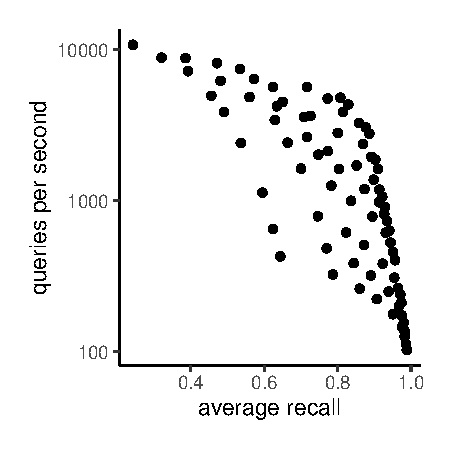
\includegraphics[width=\textwidth]{submissions/Matteo2023/figures/all_params.pdf}
		\caption{Recall/qps performance of several parameter combinations of
			HNSW on the Glove dataset.\label{matteo_fig:allparams}}
	\end{minipage}
	\hfill
	\begin{minipage}{.4\textwidth}
		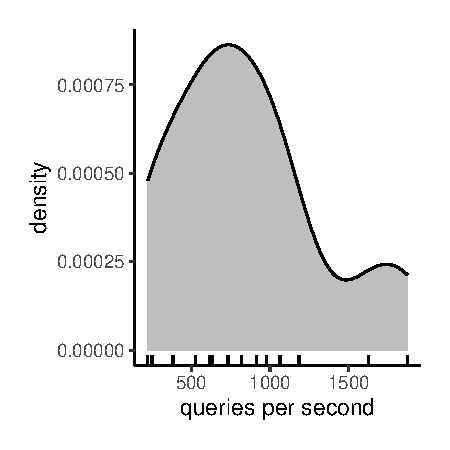
\includegraphics[width=\textwidth]{submissions/Matteo2023/figures/distribution_qps.pdf}
		\caption{Distribution of queries per second of several parameter
			combinations of HNSW achieving at least recall
			0.9.\label{matteo_fig:distribution-qps}}
	\end{minipage}
\end{figure}

Most of the times, the metrics considered for approximate
nearest neighbor queries are the query throughput and the average recall.
The query throughput---or equivalently the query time---are
however very dependent on the implementation, and are thus
measuring the performance of the implementation, rather than assessing the
merits of the underlying algorithm~\cite{DBLP:journals/kais/KriegelSZ17}.

While the actual performance of an implementation is what people are most
interested in, considering other metrics can give further insights into the
behavior of an algorithm. For instance, the number of distance
computations performed can indicate how effective an approach is at reducing
the amount of work to be performed. The interplay between the number of
distance computations and the actual running time is also of interest: a linear
scan through compressed points using product quantization may be faster than a more
sophisticated index due to better use of the cache, despite carrying out more distance
computations.
As highlighted in~\cite{DBLP:journals/corr/abs-2305-04359}, this is for example true for clustering-based
approaches compared to graph-based approaches in million-scale settings.
While the latter only carry out a fraction of distance computations, the more efficient memory layout of clustering-based approaches can make up for the additional calculations.


Furthermore, the index size and the index construction time are important
metrics to complement the execution speed.


\subsection{Selecting parameters}

Many papers evaluate the proposed method by comparing with a few state of
the art approaches, using a few configurations for each.
Some papers use just a single configuration for the baseline,
namely the default one provided by the implementation or the ones discussed in the associated publication.
This approach can however lead to misleading comparisons, in that the
performance of many approaches varies wildly in response to parameter
changes, and differently across datasets.

For instance, HNSW is a commonly used baseline to compare with, and in many
cases only a few parameter combinations are tested.
Figure~\ref{matteo_fig:allparams} reports the results---in terms of average recall
and queries per second---of answering 5\,000 queries on
\texttt{glove-100-angular}\footnote{\url{http://ann-benchmarks.com/glove-100-angular.hdf5}}
using HNSW in the implementation provided by the FAISS library~\cite{DBLP:journals/tbd/JohnsonDJ21}.
The index building parameters being used are
$M \in \{4,8,12,16,24,36,48,64,96\}$ and $efConstruction = 500$; the search parameters are varied in the range
$ef \in \{10, 20, 40, 80, 120, 200, 400, 600, 800\}$.
As one can observe, the outcomes vary wildly, both in terms of recall and
in terms of query throughput. As such, using only a single parameter
configuration as a baseline for comparison is very likely to result in
suboptimal performance for the baseline itself. In this case we consider HNSW
due to its popularity, but the same behavior can be observed with most
approaches.

Even fixing a target recall and focusing on a single configuration
achieving it does not make the performance more stable across parameter
configurations. Figure~\ref{matteo_fig:distribution-qps} shows the distribution of
the query throughput for all the aforementioned configurations that result
in an average recall between 0.9 and 0.95. As we can see, the difference
between the slowest and the fastest configurations is about two orders of
magnitude.

\subsection{Making workloads explicit}

Many papers describe which datasets are part of their experimental section and
then make a generic statement along the lines of \emph{$n$ queries are run from
	the dataset}. The reader is then left to conjecture that possibly queries are
sampled at random from the dataset. However, it has been
shown~\cite{DBLP:journals/is/AumullerC21} that the practical performance of
queries is greatly influenced by the intrinsic dimensionality of the queries
themselves. Some works already address explicitly
workloads with different
difficulties~\cite{DBLP:journals/vldb/ZoumpatianosLIP18,DBLP:journals/pvldb/EchihabiFZPB22}.

We therefore suggest to explicitly design query workloads that span a different
range of difficulties, thus allowing to assess the performance of the
approaches under test in finer detail. We provide Python code to compute
intrinsic dimensionality measures of workloads at the following public
repository: \url{https://github.com/Cecca/workloads-difficulty}.


\subsection{Dangers of reporting on averages}
\begin{figure}
	\centering
	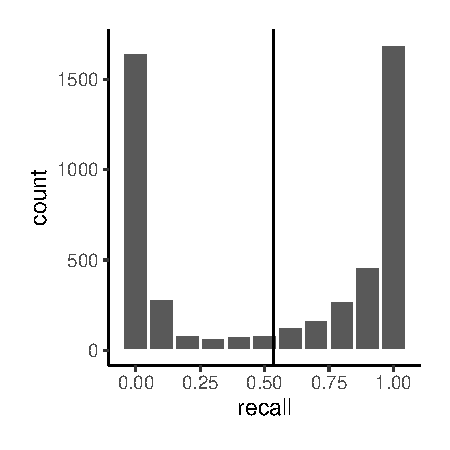
\includegraphics[width=0.4\textwidth]{submissions/Matteo2023/figures/hist_recall.pdf}
	\caption{Histogram of the recall of single queries for a configuration
		of HNSW achieving \emph{average} recall 0.55.\label{matteo_fig:hist-recall}}
\end{figure}

In the previous section we considered the average recall of 5\,000 queries
as a performance indicator.
This can be misleading at times, and hide interesting behavior.

Consider again HNSW. Figure~\ref{matteo_fig:hist-recall} reports the histogram of
the recalls of individual queries of a run attaining average recall
$\approx 0.55$\footnote{
	Using the \texttt{faiss} implementation of HNSW, with $efConstruction = 500$,
	$M = 16$ and $ef = 10$.
	Queries are the ones provided in the \texttt{glove-100-angular.hdf5} file from ANN-benchmarks.
}.
Strikingly, almost a third of the queries have recall 0, and a third
of the queries have recall 1. In this case considering the average hides
this bimodal behavior that may have important practical implications.

Therefore, we suggest to consider the distribution of the performance of
individual queries, rather than drawing conclusions based on averages alone.

\subsection{Implementation accessibility}

The possibility to access the implementation backing the findings reported in
any paper is of paramount importance for the community to verify and build upon
results.
Fortunately, in recent years the number of papers in nearest neighbor search that
make their code accessible (usually as a Git repository hosted on online services
such as GitHub or BitBucket) increased significantly.

Still, we note that code accessibility can be improved further. In some case,
the code linked to a paper fails to compile following the instructions, most
often due to differences between the environments of the code's author and the
reader. Among the many solutions to this problem, we believe the most
straightforward is to pair the code with container environments such as
Docker~\cite{DBLP:journals/sigops/Boettiger15} or
Singularity~\cite{singularity}. Doing so also makes for an easier integration
in existing benchmarking efforts, which often leverage containers in their
infrastructure~\cite{DBLP:journals/is/AumullerBF20}.

\section{New approaches to ANN search}
\label{matteo_sec:new:approaches}

Having covered general approaches to high-dimensional indexing and remarks on benchmarking efforts, we will now focus on recent work.
In the context of this overview paper, we report on approaches that appeared after the publication of the benchmarking paper~\cite{DBLP:journals/is/AumullerBF20}.

\subsection{Hashing-based Approaches}

Recent works based on hashing have focused on extending classic LSH techniques
by using new data structures, new query procedures, and by incorporating
information from the data and query distribution.

\textsc{PUFFINN}~\cite{DBLP:conf/esa/0001CPV19} is an approach whose goal
is to address approximate $k$-nearest neighbor queries while providing theoretical
guarantees on the failure probability. In order to do so, it leverages
the theoretical framework of Locality Sensitive Hashing
(LSH)~\cite{DBLP:conf/sequences/Broder97,DBLP:journals/toc/Har-PeledIM12}.
While providing theoretical
guarantees, LSH is known to have many parameters, whose setting is
crucial to achieve good performance. To overcome this issue,
\textsc{PUFFINN} adopts an \emph{adaptive} approach based on the LSH forest trie data structure~\cite{DBLP:conf/www/BawaCG05}.

\textsc{PM-LSH}~\cite{DBLP:journals/vldb/ZhengZWNLJ22}
% \footnote{Code: \url{}} 
is an approach
focusing on $L_p$ norms. Their key idea is as follows.
A dimensionality reduction using the Johnson-Lindenstrauss transform is applied to project each point into a lower-dimensional space.
The transformed points are then indexed by means of a
PM-tree~\cite{DBLP:conf/dasfaa/SkopalPS05}. Queries are then carried out
by performing several range queries on the PM-tree. While this approach
is reminiscent of the earlier SRS approach~\cite{DBLP:journals/pvldb/SunWQZL14},
there is a somehow subtle difference. Where SRS runs $k$-NN queries in
the projected space, which may suffer from the inaccuracy introduced by
the projection (i.e. the second nearest neighbor in the projected space
might not be the best candidate in the original space) PM-LSH runs a
sequence of range queries, which they demonstrate to be more accurate.

\textsc{FARGO}
% \footnote{Code:
% 	\url{https://github.com/Jacyhust/FARGO}}
~\cite{DBLP:journals/pvldb/ZhaoZYLXZJ23}
focuses on the Maximum Inner Product Search problem (MIPS). In order to
apply LSH to the MIPS problem, the paper proposes an asymmetric
transformation of data and queries so that all data points have the same
norm, while retaining the original inner products with the queries. Then
data points are indexed using LSH, and queried using a multi-probing approach.

\textsc{CEO-MIPS}~\cite{DBLP:conf/kdd/Pham21} targets the MIPS problem as well,
by performing several Gaussian random projections of the data and the queries.
By leveraging the theory of concomitants of extreme order statistics,
\textsc{CEO-MIPS} considers among all the projections of the query only the one
with maximum value. If the $i$-th projection maximizes the absolute inner product, then it considers as candidates the data points
whose $i$-th projection is large. The paper describes several variants of the
approach that reduce the space usage.

\textsc{FALCONN++}~\cite{DBLP:conf/nips/PhamL22} improves on the
Cross-Polytope-based hashing used in the FALCONN
library~\cite{DBLP:conf/nips/AndoniILRS15}.
The main insight is that
mapping a data point into a bucket based on the random vector that
maximizes the inner product (crosspolytope hashing), can also be used as an estimator of the
distance between the point and the query vector, similarly to~\cite{DBLP:conf/kdd/Pham21}.
The paper proposes a
threshold for the inner product to keep a point in a bucket, otherwise it
is filtered away. This is the first practical implementation using the
locality-sensitive filtering technique proposed by Andoni et
al.~\cite{DBLP:conf/soda/AndoniLRW17} and by
Christiani~\cite{DBLP:conf/soda/Christiani17} in the context of
approximate nearest neighbor search. We note that Rashtchian et
al.~\cite{DBLP:conf/www/RashtchianSW20} used this framework for computing similarity joins for skewed data.

\textsc{LSH-co-substring}
% \footnote{Code is available
% 	\url{https://github.com/1flei/lccs-lsh}}
~\cite{DBLP:conf/sigmod/LeiHKT20}
seeks to overcome one of the main hurdles of using LSH, that is selecting
the number of repetitions. The key idea is that, instead of performing
$L$ repetitions of the LSH scheme, each vector is associated with a
string of hash values of length $m$. Then, instead of defining buckets, a
query looks for the hash strings with the longest colliding subsequence,
allowing wraparounds at the string boundaries. The experimental analysis
shows that the approach has an edge over other LSH-based approaches in
terms of query time at a given recall, with markedly smaller index sizes.


\textsc{LSH-APG}
% \footnote{Code: \url{ https://github.com/Jacyhust/LSH-APG
% 	}}
~\cite{DBLP:journals/pvldb/ZhaoTHZZ23} aspires to blend together LSH
and graph-based approaches. In particular, LSH is used to speed up the
construction of a graph-based index. At query time, LSH is again used
to select a few entry points into the graph; these are then used to
handle the search for the best query answers. Experiments show that
LSH-APG has a larger index than graph-based methods, but such index can
indeed be constructed much faster. Furthermore, the query performance at
fixed parameters is shown to be better than other graph-based approaches.

\textsc{DB-LSH}
% \footnote{Code:
% 	\url{https://github.com/Jacyhust/DB-LSH}}
~\cite{DBLP:conf/icde/TianZZ22}
employs a \emph{dynamic bucketing} scheme, modifying the classic LSH
approach, to answer range queries. The traditional LSH approach for the
Euclidean distance requires to project points onto a random direction,
and then to bucket the projections \emph{at indexing time} to build the
hash codes. In \textsc{DB-LSH} such quantization is deferred to
\emph{query time}, so to be able to center the buckets around the query.
In particular, at index time the random projections of the dataset points
are indexed in an R*-tree. At query time, the R*-tree is used to
answer a sequence of (rectangular) range searches, that are equivalent to
dynamically bucketing the hash values around the query.

\textsc{HD-index}~\cite{DBLP:journals/pvldb/AroraSK018} answers
approximate $k$-nearest neighbor queries with the aim to use less space
than LSH. The core idea is to partition the dataset with a regular grid,
which is then traversed using a space-filling curve (such as Hilbert of
Z-order). Points are then inserted in a tree-like data structure using
their position along the space filling curve as keys. The rationale
is that points that are close in a geometric sense are also close along
the space filling curve. The experiments reported in the paper show that,
compared to baselines
the \textsc{HD-index} answers queries with a
better Mean Average Precision, in a shorter time.


\subsection{Graph-based approaches}

Graph-based approaches offer among the largest variety of known methods, see
for example the survey paper by Wang et
al.~\cite{DBLP:journals/pvldb/WangXY021}. In general, recent works have focused
on enabling the use of graph-based approaches on larger-than-memory data,
on addressing the issue of indexing time, and on designing pruning/refinement strategies for the graph building process.

\textsc{DiskANN~\cite{DBLP:conf/nips/SubramanyaDSKK19}}
targets approximate nearest neighbor search in an external memory setting,
where the size of the dataset makes it impossible to store the index and the
data entirely in memory.
Therefore, the main aim is to develop an index that minimizes the number of
disk reads per query to amortize the disk latency.
To this end, \textsc{DiskANN} refines a random
$k$-regular graph using iterated beam searches from a central graph node,
the medoid. It refines the graph in two steps with different pruning
values. In difference to HNSW, no hierarchy is employed.

\textsc{ELPIS}~\cite{DBLP:journals/pvldb/AziziEP23} tackles one of the main
issues of graph-based approaches, which is the index construction time. It
does so by first partitioning the datasets using a tree-based data
structure, and then by using HNSW to build graphs on the leaves. As such,
the graph construction is carried out in parallel on smaller subsets of the
data. This leads to a faster index construction and to a smaller index as
well.
In particular, \textsc{ELPIS} builds its tree by employing dimensionality
reduction techniques borrowed from the \emph{data series} community,
observing that a high-dimensional vector can be considered as an instance of
a data series.

Dobson et al.~\cite{DBLP:journals/corr/abs-2305-04359} give a detailed account on scaling graph-based nearest neighbor search implementations to billion-scale datasets.
In particular, they describe parallelization techniques to deal with the potential data dependencies that can occur during the parallel insertion of points.


\subsection{Clustering-based approaches}

\textsc{\textsc{SCANN}~\cite{DBLP:conf/icml/GuoSLGSCK20}} extends the
standard inverted file index based on (hierarchical) $k$-means
clustering, designed for inner product spaces. Their motivation is that
$\ell_2$-based $k$-means clustering may favor centroids that do not
preserve the ordering under inner product similarity. To mitigate this
issue, they propose an anisotropic quantization technique which is more
accurate for inner product similarity. A significant ingredient to
SCANN's performance is a very efficient product quantization
implementation based on SIMD instructions as described by Andre et
al.~\cite{DBLP:journals/pami/AndreKS21}.
Sun et al.~\cite{DBLP:conf/iclr/SunGK23} extend the approach with an efficient hyper-parameter selection technique.


\subsection{Learning-based approaches}

Algorithms with predictions~\cite{DBLP:conf/sigmod/KraskaBCDP18} is a
recent trend in the development of algorithms and data structures. The idea is that an
oracle, for example a machine learning model, gives predictions for data
that is stored in the data structure. An overview over progress in this
field in general is given by Mitzenmacher and
Vassilvitskii~\cite{DBLP:journals/cacm/MitzenmacherV22}.
A thorough survey of deep learning-based methods for approximate nearest neighbor search is given in~\cite{DBLP:journals/tkde/LiWZWFLW23}.

In the context of ANN search, two main research directions are (i) using a machine learning model to guide the candidate generation and (ii) using a machine learning model to set adaptive stopping criteria in a traditional data structure.
In the former, the indexing part is augmented with a machine learning model; in the latter, the search phase is augmented using such a model.

\textsc{ANN as Multilabel Classification} by Hyvönen et
al.~\cite{DBLP:conf/nips/HyvonenJR22} proposes to formulate the following
multi-label classification problem: Given $S \subseteq \mathcal{X}$ and
$x \in \mathcal{X}$, let $y_i = [p_i \text{ is a $k$-NN of $x$ in $S$}]$.
Thus, the (high-dimensional) label $y = (y_1, \ldots, y_n)$ represents
the set of $k$ nearest neighbors of $x$. Given these pairs $\{(x^{(i)},
	y^{(i)})\}_{1 \leq i \leq n}$, we can train a classifier for this
multi-label classification problem. Applied to space partitioning nearest
neighbor search algorithms, such as trees, LSH, or clustering-based
variants, the authors show that the pre-dominant approach that collects the
points that fall into the same part of the partition (i.e., a leaf or a
bucket) is not the \emph{natural classifier} for the multi-label
classification problem. Instead, one should use a majority vote based on
groundtruth labels $y$ of these points to decide on the candidates to
check.

\textsc{NeuralLSH}~\cite{DBLP:conf/iclr/DongIRW20} proposes to build the
$k$-NN graph on the dataset $S$, and find a balanced partition of this
graph into $m$ disjoint parts. These $m$ parts form the $m$ buckets of
the data structure. The label of a point $x$ is an $m$-bit string, where
the $i$-th bit is set if $x$ has a $k$-NN in part $i$ of the graph. The labeling
is learned by means of a neural network, and the search is guided by
predicting bucket probabilities using the neural network, and checking
all buckets in sorted order, thresholding at a certain value.

\textsc{BLISS}~\cite{DBLP:conf/kdd/GuptaMSS22} applies iterative
repartitioning by \emph{learning the bucket assignment} and
\emph{redistributing points} according to the learned assignments, in rounds. More
precisely, data points are split up at random into $B$ groups/buckets.
The label of a data point $x$ is a length-$B$ bit string; label $i \in
	\{1, \ldots, B\}$ is set if the nearest neighbor of $x$ is in group $i$.
After learning the assignment, a prediction step is carried out for each
data point, the top-$K$ buckets with the highest probability are
retrieved, and the data point is moved to the least loaded bucket among
these top-$K$. The process is repeated $R$ times independently.
Experimentally, a small value of $R$ is sufficient, and $B$ is set to
roughly $\sqrt{n}$.


\textsc{Learning to Hash, Robustly}~\cite{DBLP:conf/icml/AndoniB22} proposes a
learned LSH function for binary data under Hamming distance. In particular,
rather than sampling bit-coordinates uniformly at random as in the standard LSH
scheme, the paper describes a method to optimize the probability distribution
over coordinates, for the given dataset. In contrast to the approaches
mentioned above, they can guarantee worst-case running time comparable to the
best known theoretical approaches, while being able to adapt to the difficulty
of a query dynamically.

Li et al.~\cite{DBLP:conf/sigmod/LiZAH20} note that most approaches using
indexes to reduce the number of candidates to evaluate do not adapt to the
\emph{difficulty} of a query, i.e., use the same stopping condition for all
queries. The consequence is that to achieve a good recall a conservative
stopping condition needs to be used, thus hurting the performance of easier
queries. Therefore, they develop a prediction pipeline based on gradient
boosting decision trees, allowing the implementation of an adaptive stopping
condition. Such an adaptive stopping condition is then implemented in the IVF and
HNSW indexes, with experiments showing a general reduction in latency.


Continuing along the line of the previous paper, Zheng et
al.~\cite{DBLP:conf/icde/ZhengYHYLX0J23} focus on IVF indexes, with the aim of
setting the number of cells to probe on a per query basis. To this end, they
first modify the way data vectors are clustered, so to ensure that each cluster
has a balanced number of entries. Then they use autoencoders, trained offline
on sample queries, to estimate the number of cells to probe for a query.

\subsection{Refining Candidates}

In the context of nearest neighbor search, an important ingredient of the system pipeline is the refinement of a set of candidates.
To this end, one wants to compress vectors in a way such that points \emph{likely to not be part} of the $k$ nearest neighbors are to be excluded without incurring an exact distance computation.
A general overview of the techniques is given by Pagh in~\cite{DBLP:reference/bdt/Pagh19}.
The main technique used is Product Quantization as introduced by Jegou et al.~\cite{DBLP:journals/pami/JegouDS11}.
An overview over this technique and its variants is given by Matsui et al.~\cite{matsui2018survey}.

\textsc{FINGER}~\cite{DBLP:conf/www/ChenCJYDH23} aims at improving the speed
at which nearest neighbor graphs are traversed. The key observation is that
during traversals most of the distances do not need to be computed exactly.
Therefore, the paper proposes an estimation method to quickly estimate distances
that can be used to improve the performance of any graph-based nearest
neighbor algorithm. To showcase the performance of the approach, the paper
integrates it in an HNSW implementation.

\textsc{ADSampling}~\cite{DBLP:journals/pacmmod/GaoL23} aims at optimizing one
of the most basic operations in nearest neighbor search: the distance
comparison operation, which given a pair of points returns whether the points'
distance is above or below a given threshold. First, the same random rotation
is applied to each point. Then, given two vectors their distance is computed by
considering the rotated dimensions one at a time, in a progressive sampling
fashion, conducting a statistical hypothesis test on whether the two vectors
are closer or farther than the threshold.

\textsc{LVQ}~\cite{AuguerrebereBSHT23} describes a locally-adaptive vector quantization technique, which uses scalar quantization with individual lower and upper bounds on the coordinate values.
Employed in a graph-based index, the authors show compelling performance up to billion-scale datasets.

\section{Trends}
\label{matteo_sec:trends}

\subsection{Billion-Scale ANN search}

Scaling ANN search to billion-scale datasets has been one of the core research directions of the past years.
In particular, this is supported by the availability of diverse datasets through the NeurIPS 2021 Billion-Scale ANN challenge~\cite{DBLP:conf/nips/SimhadriWADBBCH21} and other large datasets such as Laion5B~\cite{DBLP:conf/nips/SchuhmannBVGWCC22}.
On this scale, index construction time and index size pose the most challenging part of the indexing pipeline.
Dobson et al.~\cite{DBLP:journals/corr/abs-2305-04359} provide an empirical comparison of the scaling of different approaches from million to billion scale, focusing primarily on graph-based approaches. They discuss different parallelization strategies to efficiently parallelize the index construction and the (batched) search.
They conclude that graph-based nearest neighbor search performs best on billion-scale datasets in the high recall regime.
In terms of index building times and index size, clustering- and hashing-based approaches were shown to be competitive.

\subsection{New Tasks in ANN Search}

In the following we describe extension of nearest neighbor search targeted towards real-world applications.

\paragraph{Filtered Search} When data vectors are associated with some metadata, for example for the \textsc{Yfcc-100M}~\cite{DBLP:journals/cacm/ThomeeSFENPBL16} dataset or the \textsc{Laion5B} dataset~\cite{DBLP:conf/nips/SchuhmannBVGWCC22}, a natural extension to $k$-NN search is to incorporate the metadata into the query.
Technically, each data vector is associated with a bag-of-words representation of its tags. The query vector additionally has tags $t_1,\ldots,t_T$, and the task is to find the (approximate) $k$-NN among all points in the dataset that contain the query's tags. A graph-based solution to this problem is described by Gollapudi et al.~\cite{DBLP:conf/www/GollapudiKSKBRL23-filter}.

\paragraph{Out-of-Distribution Queries}
A common scenario in modern approximate nearest neighbor search is that data and query vectors originate from different distributions, but are embedded into the same space.
For example, the Yandex \textsc{text2image} dataset~\cite{DBLP:conf/nips/SimhadriWADBBCH21} consists of image embeddings produced by the Se-ResNext-101 model described by Hu et al.~\cite{DBLP:conf/cvpr/HuSS18}, while queries are textual embeddings produced by a variant of the DSSM model by Huang et al.~\cite{DBLP:conf/cikm/HuangHGDAH13}.
As described in~\cite{DBLP:conf/nips/SimhadriWADBBCH21}, the mapping to the shared 200-dimensional real valued vectors under inner product similarity is learned via minimizing a variant of the triplet loss using clickthrough data.
A novel approach to explicitly deal with out-of-distribution queries is described in~\cite{DBLP:journals/corr/abs-2211-12850-ood}.
As pointed out in~\cite{DBLP:journals/corr/abs-2305-04359}, cluster- and LSH-based approaches are particularly affected by these changes in distribution.


\paragraph{Streaming Search}
A particular challenge in the index building process is to maintain an index over dynamic insertions and deletions.
Technically, a stream of \emph{add}, \emph{delete}, \emph{search} operations is given, where each search is supposed to return the approximate $k$-nearest neighbors of all the elements that are in the index according to the \emph{add} and \emph{delete} operations.
Simhadri~\footnote{\url{https://harsha-simhadri.org/pubs/ANNS-talk-Sep22.pptx}, (accessed on Sept 25, 2023.)} describes different applications of this setting.
For example, for web search the index may contain roughly a trillion vectors and has to handle billions of updates per day.
Searches have to be handled at a latency of at most 10 milliseconds with a throughput of 10,000-100,000 queries per second.
Naïve solutions such as placing tombstones for deleted items quickly degrade performance, as would a complete rebuild of the index in a given interval size.
Singh et al.~\cite{DBLP:journals/corr/abs-2105-09613-stream} describe a graph-based approach to handle this issue and show competitive performance to the non-stream setting, and a big improvement over previous LSH-based approaches~\cite{DBLP:journals/pvldb/SundaramTSMIMD13}.
Their system handles thousands of add/delete operations per second while maintaining high recall/throughput comparable to the non-streaming setting.
A special case of this dynamic setting is \emph{content drift}, which was studied by Baranchuk et al.~\cite{DBLP:journals/corr/abs-2308-02752-drift}.


\subsection{Conclusions}

In recent years, the field of approximate nearest
neighbor search has witnessed an exciting surge in the development of new approaches and the refinement of existing methods. Alongside the
traditional $k$-nearest neighbor setting, new tasks are emerging:
queries can incorporate different metadata such as tags, an index has to be kept over a dynamic stream of search, insert, and remove operations, or queries might arise from a different
distribution than the data points. Moreover, the scale of today's datasets has reached billions of data points, requiring unprecedented scalability while retaining
accuracy.

Given the practical relevance of the problem, it is crucial that new approaches
are benchmarked thoroughly. Given the effort needed to set up a benchmarking
infrastructure, we invite the research community to adopt and improve shared benchmarks which avoid the pitfalls that commonly affect experimental evaluations.



\paragraph{Acknowledgements:} Martin Aumüller thanks Yusuke Matsui for insightful discussions. He also thanks his collaborators
organizing and working on approximate nearest neighbor search challenges
\cite{DBLP:conf/nips/SimhadriWADBBCH21,sisap23challenge}, and the NeurIPS'23 challenge\footnote{\url{https://big-ann-benchmarks.com/}}. This research was supported by the Innovation Fund Denmark for the project DIREC
(9142-00001B).

\bibliographystyle{plainnat} 
\bibliography{submissions/Matteo2023/references}

\end{document}

